\begin{mydef}
	Un losange est un quadrilatère qui possède \kw{quatre côtés de même longueur}.
\end{mydef}

\begin{myprops}
	\textbf{Si} un quadrilatère est un losange \textbf{alors} 
	\begin{itemize}
		\item ses \kw{quatre cotés} font la \kw{même longueur};
		\item ses \kw{diagonales} ont \kw{perpendiculaires}.
	\end{itemize}
\end{myprops}

\begin{myex}
	\begin{center}
		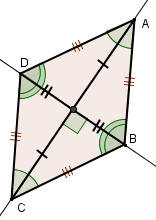
\includegraphics[scale=0.15]{losange}
	\end{center}

	ABCD est un losange donc :
 	\begin{itemize}
 		\item $AB = BC = CD = DA$ ;
 		\item $(AC) \perp (BD)$.
 	\end{itemize}	
\end{myex}